\documentclass[cmyk,a4paper,colorscheme=green,TUBStitlepage=picture]{tubsreprt}

\usepackage[utf8x]{inputenc}
\usepackage[LY1]{fontenc}
\usepackage{ngerman}
\usepackage{listings}
\lstset{basicstyle=\ttfamily}
\usepackage{xcolor}
\usepackage[colorlinks=true]{hyperref}
\usepackage{tikz} % TODO: should be RequirePackage
\usepackage{booktabs}

% Copyright 2003--2007 by Till Tantau
% Copyright 2010 by Vedran Mileti\'c
%
% This file may be distributed and/or modified
%
% 1. under the LaTeX Project Public License and/or
% 2. under the GNU Free Documentation License.
%
% See the file doc/licenses/LICENSE for more details.

% $Header: /home/vedranm/bitbucket/beamer/doc/beamerug-macros.tex,v 14743c450e2c 2010/06/17 09:25:56 rivanvx $

\def\beamer{\textsc{beamer}}
\def\pdf{\textsc{pdf}}
\def\pgfname{\textsc{pgf}}
\def\translatorname{\textsc{translator}}
\def\pstricks{\textsc{pstricks}}
\def\prosper{\textsc{prosper}}
\def\seminar{\textsc{seminar}}
\def\texpower{\textsc{texpower}}
\def\foils{\textsc{foils}}

{
  \makeatletter
  \global\let\myempty=\@empty
  \global\let\mygobble=\@gobble
  \catcode`\@=12
  \gdef\getridofats#1@#2\relax{%
    \def\getridtest{#2}%
    \ifx\getridtest\myempty%
      \expandafter\def\expandafter\strippedat\expandafter{\strippedat#1}
    \else%
      \expandafter\def\expandafter\strippedat\expandafter{\strippedat#1\protect\printanat}
      \getridofats#2\relax%
    \fi%
  }

  \gdef\removeats#1{%
    \let\strippedat\myempty%
    \edef\strippedtext{\stripcommand#1}%
    \expandafter\getridofats\strippedtext @\relax%
  }

  \gdef\stripcommand#1{\expandafter\@gobble\string#1}
}

\providecommand\href[2]{\texttt{#1}}

\def\printanat{\char`\@}

\def\declare#1{{\color{red!75!black}#1}}
%\def\declare{\afterassignment\translatormanualdeclare\let\next=}
%\def\translatormanualdeclare{\ifx\next\bgroup\bgroup\color{red!75!black}\else{\color{red!75!black}\next}\fi}

\def\command#1{\list{}{\leftmargin=2em\itemindent-\leftmargin\def\makelabel##1{\hss##1}}%
\item\extractcommand#1@\par\topsep=0pt}
\def\endcommand{\endlist}
\def\extractcommand#1#2@{\strut\declare{\texttt{\string#1}}#2%
  \index{\stripcommand#1@\protect\myprintocmmand{\stripcommand#1}}}

%\let\textoken=\command
%\let\endtextoken=\endcommand

\def\myprintocmmand#1{\texttt{\char`\\#1}}

\def\example{\par\smallskip\noindent\textit{Beispiel: }}
\def\themeauthor{\par\smallskip\noindent\textit{Theme author: }}

\def\environment#1{\list{}{\leftmargin=2em\itemindent-\leftmargin\def\makelabel##1{\hss##1}}%
\extractenvironement#1@\par\topsep=0pt}
\def\endenvironment{\endlist}
\def\extractenvironement#1#2@{%
\item{{\ttfamily\char`\\begin\char`\{\declare{#1}\char`\}}#2}%
  {\itemsep=0pt\parskip=0pt\item{\meta{environment contents}}%
  \item{\ttfamily\char`\\end\char`\{\declare{#1}\char`\}}}%
  \index{#1@\protect\texttt{#1} environment}%
  \index{Environments!#1@\protect\texttt{#1}}}

\def\classoption#1{\list{}{\leftmargin=2em\itemindent-\leftmargin\def\makelabel##1{\hss##1}}%
\item{{\ttfamily\char`\\documentclass[\declare{#1}]\char`\{beamer\char`\}}}
  \index{#1@\protect\texttt{#1} class option}%
  \index{Class options for \textsc{beamer}!#1@\protect\texttt{#1}}%
  \par\topsep=0pt}
\def\endclassoption{\endlist}


\newcommand\beameroption[2]{\list{}{\leftmargin=2em\itemindent-\leftmargin\def\makelabel##1{\hss##1}}%
\item{{\ttfamily\char`\\setbeameroption\char`\{\declare{#1}{\normalfont\opt{#2}}\char`\}}}
  \index{#1@\protect\texttt{#1} beamer option}%
  \index{Beamer options!#1@\protect\texttt{#1}}%
  \par\topsep=0pt}
\def\endbeameroption{\endlist}


\def\smallpackage{\vbox\bgroup\package}
\def\endsmallpackage{\egroup\endpackage}

\def\package#1{\list{}{\leftmargin=2em\itemindent-\leftmargin\def\makelabel##1{\hss##1}}%
\extracttheme#1@usepackage@package@Packages@\par\topsep=0pt}
\def\endpackage{\endlist}
%\def\extracttheme#1#2@{%
%\item{{{\ttfamily\char`\\usepackage}#2{\ttfamily\char`\{\declare{#1}\char`\}}}}}

\def\theme#1#2#3#4{\list{}{\leftmargin=2em\itemindent-\leftmargin\def\makelabel##1{\hss##1}}%
\extracttheme#2@#1@#3@#4@\par\topsep=0pt}
\def\endtheme{\endlist}
\def\extracttheme#1#2@#3@#4@#5@{%
\item{{{\ttfamily\char`\\#3}#2{\ttfamily\char`\{\declare{#1}\char`\}}}}%
  \index{#1@\protect\texttt{#1} #4}%
  \index{#5!#1@\protect\texttt{#1}}
}

\def\class#1{\list{}{\leftmargin=2em\itemindent-\leftmargin\def\makelabel##1{\hss##1}}%
\extractclass#1@\par\topsep=0pt}
\def\endclass{\endlist}
\def\extractclass#1#2@{%
\item{{{\ttfamily\char`\\documentclass}#2{\ttfamily\char`\{\declare{#1}\char`\}}}}%
  \index{#1@\protect\texttt{#1} class}%
  \index{Classes!#1@\protect\texttt{#1}}}

\def\typesetsol#1{\texttt{\def\_{\char`\_}#1}}

\def\solution#1{\list{}{\leftmargin=2em\itemindent-\leftmargin\def\makelabel##1{\hss##1}}%
\item \textbf{Solution Template }\declare{\typesetsol{#1}}\par\topsep=0pt%
  \index{#1@\protect\typesetsol{#1} solution}%
  \index{Solutions!#1@\protect\typesetsol{#1}}}
\def\endsolution{\endlist}

\def\template#1{\list{}{\leftmargin=2em\itemindent-\leftmargin\def\makelabel##1{\hss##1}}%
\item {\ttfamily\char`\\setbeamertemplate\char`\{\declare{#1}\char`\}}\oarg{options}\opt{\meta{args}}\par\topsep=0pt}
\def\endtemplate{\endlist}
\newenvironment{template*}[1]{\list{}{\leftmargin=2em\itemindent-\leftmargin\def\makelabel##1{\hss##1}}%
\item \leavevmode\llap{\color{blue}\vtop
    to0pt{\llap{\textsc{appear-\!}}\vskip-3pt\llap{\textsc{ance}}\vss}\ \ }{\ttfamily\char`\\setbeamertemplate\char`\{\declare{#1}\char`\}}\oarg{options}\opt{\meta{args}}\par\topsep=0pt}
{\endlist}

\newenvironment{element}[4]{\list{}{\leftmargin=2em\itemindent-\leftmargin\def\makelabel##1{\hss##1}}%
\item \textbf{\ifx#2\semiyes Parent Beamer-Template\else%
    Beamer\applier#2{-Template}\applier#3{\applier#2{/}-Color}\applier#4{\ifx#2\yes/\else\ifx#3\yes/\fi\fi
      -Font}\fi}
    {\ttfamily{\declare{#1}}}\par\topsep=0pt%
  \edef\parameters{%
    \ifx#2\semiyes parent template\else%
    \applier#2{template}\applier#3{\applier#2{/}color}\applier#4{\ifx#2\yes/\else\ifx#3\yes/\fi\fi font}\fi}
  \index{#1@\protect\texttt{#1} \parameters}%
  \applier#2{\index{Beamer templates!#1@\protect\texttt{#1}}}%
  \applier#3{\index{Beamer colors!#1@\protect\texttt{#1}}}%
  \applier#4{\index{Beamer fonts!#1@\protect\texttt{#1}}}%
}
{\endlist}

\def\applier#1#2{\ifx#1\yes#2\fi}

\def\templateoptions{\par
  The following template options are predefined:
  \begin{itemize}}
\def\endtemplateoptions{\end{itemize}}

\def\itemoption#1#2{\item {\texttt{[\declare{#1}]}}#2}

%\def\itemoption#1{\item \declare{\texttt{#1}}%
%  \indexoption{#1}%
%}

%\def\indexoption#1{%
%  \index{#1@\protect\texttt{#1} option}%
%  \index{Options!#1@\protect\texttt{#1}}%
%}

\def\yes{\hbox to .6cm{\ding{51}\hfil}}
\def\semiyes{\hbox to .6cm{(\ding{51})\hfil}}
\def\no{\hbox to .6cm{\ding{55}\hfil}}

\def\choosecol#1{}%\ifx#1\yes\color{green!50!black}\else\color{red!50!black}\fi}

\def\templatefontcolor#1#2#3#4{%
  \item\declare{\texttt{#1}}\hfill%
  {\choosecol#2Template #2} {\choosecol#3Color #3} {\choosecol#4Font #4}\par}

\def\fontparents#1{Font parents: \texttt{#1}\par}
\def\colorparents#1{Color parents: \texttt{#1}\par}
\def\colorfontparents#1{Color/font parents: \texttt{#1}\par}

\def\templateinserts{\begin{itemize}}
\def\endtemplateinserts{\end{itemize}}

\def\iteminsert#1{\item {\texttt{\declare{\string#1}}}%
  \index{Inserts!\stripcommand#1@\protect\myprintocmmand{\stripcommand#1}}}

\newcommand\opt[1]{{\color{black!50!green}#1}}
\newcommand\oarg[1]{\opt{{\ttfamily[}\meta{#1}{\ttfamily]}}}
\newcommand\ooarg[1]{{\ttfamily[}\meta{#1}{\ttfamily]}}
\newcommand\sarg[1]{\opt{{\ttfamily\char`\<}\meta{#1}{\ttfamily\char`\>}}}
\newcommand\ssarg[1]{{\ttfamily\char`\<}\meta{#1}{\ttfamily\char`\>}}

%\def\opt{\afterassignment\translatormanualopt\let\next=}
\def\translatormanualopt{\ifx\next\bgroup\bgroup\color{black!50!green}\else{\color{black!50!green}\next}\fi}

\providecommand{\LyX}{L\kern-.1667em\lower.25em\hbox{Y}\kern-.125emX\@}

\newcommand{\beamernote}{\par\smallskip\noindent\llap{\color{blue}\vtop to0pt{\llap{\textsc{presen-\!}}\vskip-3pt\llap{\textsc{tation}}\vss}\ \ }}
\newcommand{\articlenote}{\par\smallskip\noindent\llap{\color{blue}\textsc{article}\ \ }}
\newcommand{\lyxnote}{\par\smallskip\noindent\llap{\color{blue}\textsc{lyx}\ \ }}
\newcommand{\appearancenote}{\par\smallskip\noindent\appearancenotetext}

\def\appearancenotetext{\llap{\color{blue}\vtop
    to0pt{\llap{\textsc{appear-\!}}\vskip-3pt\llap{\textsc{ance}}\vss}\ \ }}

\newcommand{\templatenote}{\par\smallskip\noindent\llap{\color{blue}\textsc{template}\ \ }}
\newcommand{\colornote}{\par\smallskip\noindent\llap{\color{blue}\textsc{color}\ \ }}
\newcommand{\fontnote}{\par\smallskip\noindent\llap{\color{blue}\textsc{font}\ \ }}

\newcommand{\genericthemeexample}[2][]{%
  \smallskip\par\noindent
  \pgfimage[width=.45\textwidth,page=1]{beamerug#2}\qquad\pgfimage[width=.45\textwidth,page=2]{beamerug#2}
  \smallskip\par}
\newenvironment{themeexample}[2][]
{\begin{theme}{usetheme}{{#2}#1}{presentation theme}{Presentation themes}
    \example\genericthemeexample{theme#2}
  }
{\end{theme}}
\newenvironment{innerthemeexample}[2][]
{\begin{theme}{useinnertheme}{{#2}#1}{inner theme}{Inner themes}
    \example\genericthemeexample{innertheme#2}
  }
{\end{theme}}
\newenvironment{outerthemeexample}[2][]
{\begin{theme}{useoutertheme}{{#2}#1}{outer theme}{Outer themes}
    \example\genericthemeexample{outertheme#2}
  }
{\end{theme}}
\newenvironment{colorthemeexample}[2][]
{\begin{theme}{usecolortheme}{{#2}#1}{color theme}{Color themes}
    \example\genericthemeexample{colortheme#2}
  }
{\end{theme}}
\newenvironment{fontthemeexample}[2][]
{\begin{theme}{usefonttheme}{{#2}#1}{font theme}{Font themes}
    \example\genericthemeexample{fonttheme#2}
  }
{\end{theme}}
\newenvironment{fontthemeexample*}[2][]
{\begin{theme}{usefonttheme}{{#2}#1}{font theme}{Font themes}}
{\end{theme}}

\def\partname{Part}

\colorlet{examplefill}{yellow!80!black}
\definecolor{graphicbackground}{rgb}{0.96,0.96,0.8}
\definecolor{codebackground}{rgb}{0.8,0.8,1}

\newenvironment{translatormanualentry}{\list{}{\leftmargin=2em\itemindent-\leftmargin\def\makelabel##1{\hss##1}}}{\endlist}
\newcommand\translatormanualentryheadline[1]{\itemsep=0pt\parskip=0pt\item\strut#1\par\topsep=0pt}
\newcommand\translatormanualbody{\parskip3pt}


%\newenvironment{command}[1]{
%  \begin{translatormanualentry}
%    \extractcommand#1\@@
%    \translatormanualbody
%}
%{
%  \end{translatormanualentry}
%}

%\def\extractcommand#1#2\@@{%
%  \translatormanualentryheadline{\declare{\texttt{\string#1}}#2}%
%  \removeats{#1}%
%  \index{\strippedat @\protect\myprintocmmand{\strippedat}}}


\renewenvironment{environment}[1]{
  \begin{translatormanualentry}
    \extractenvironement#1\@@
    \translatormanualbody
}
{
  \end{translatormanualentry}
}

\def\extractenvironement#1#2\@@{%
  \translatormanualentryheadline{{\ttfamily\char`\\begin\char`\{\declare{#1}\char`\}}#2}%
  \translatormanualentryheadline{{\ttfamily\ \ }\meta{environment contents}}%
  \translatormanualentryheadline{{\ttfamily\char`\\end\char`\{\declare{#1}\char`\}}}%
  \index{#1@\protect\texttt{#1} environment}%
  \index{Environments!#1@\protect\texttt{#1}}}



%\newenvironment{package}[1]{
%  \begin{translatormanualentry}
%    \translatormanualentryheadline{{\ttfamily\char`\\usepackage\opt{[\meta{options}]}\char`\{\declare{#1}\char`\}}}
%    \index{#1@\protect\texttt{#1} package}%
%    \index{Packages and files!#1@\protect\texttt{#1}}%
%    \translatormanualbody
%}
%{
%  \end{translatormanualentry}
%}



\newenvironment{filedescription}[1]{
  \begin{translatormanualentry}
    \translatormanualentryheadline{File {\ttfamily\declare{#1}}}%
    \index{#1@\protect\texttt{#1} file}%
    \index{Packages and files!#1@\protect\texttt{#1}}%
    \translatormanualbody
}
{
  \end{translatormanualentry}
}


\newenvironment{packageoption}[1]{
  \begin{translatormanualentry}
    \translatormanualentryheadline{{\ttfamily\char`\\usepackage[\declare{#1}]\char`\{translator\char`\}}}
    \index{#1@\protect\texttt{#1} package option}%
    \index{Package options for \textsc{translator}!#1@\protect\texttt{#1}}%
    \translatormanualbody
}
{
  \end{translatormanualentry}
}

\makeatletter
\def\index@prologue{\section*{Index}\addcontentsline{toc}{section}{Index}
  This index only contains automatically generated entries, sorry. A good
  index should also contain carefully selected keywords.
  \bigskip
}
% \c@IndexColumns=2
%   \def\theindex{\@restonecoltrue
%     \columnseprule \z@  \columnsep 35\p@
%     \twocolumn[\index@prologue]%
%        \parindent -30pt
%        \columnsep 15pt
%        \parskip 0pt plus 1pt
%        \leftskip 30pt
%        \rightskip 0pt plus 2cm
%        \small
%        \def\@idxitem{\par}%
%     \let\item\@idxitem \ignorespaces}
%   \def\endtheindex{\onecolumn}
% \def\noindexing{\let\index=\@gobble}

\makeatother



\author{Enrico Jörns}
\title{LaTeX-Präsentationen im Corporate Design}
\institute{TU-Braunschweig}
\subject{Anleitung und Dokumentation}
% \institute{Institut für Lorem Ipsum}
% \address{123 Fakestreet \\ 1337 Notown}

\parindent0mm
\parskip\medskipamount

\begin{document}

\maketitle

\begin{abstract}
Es ist freilich nicht jedem Menschen zuzumuten, seine Präsentationen in
Powerpoint oder ähnlichen Programmen erstellen zu müssen.
Aus diesem Grund wurde viel Zeit und Mühe investiert, das Corporate-Design der
TU-Braunschweig in ein Vorlage für das \LaTeX-Beamer-Paket zu gießen.\medskip

Dabei wurde unter anderem Wert darauf gelegt, so wenig wie möglich an dem
Standardverhalten und Kommandoumfang des Beamer-Paketes zu ändern und darüber
hinaus so viel Flexibilität wie möglich und sinnvoll zu behalten.\medskip

Das Beamer-Theme stammt maßgeblich von Martin Bäker. Ebenfalls daran beteiligt
waren Mr X, Mrs Y und Enrico Jörns.%TODO...
\bigskip

Wir wünschen viel Erfolg und Freude bei der Arbeit mit der Vorlage.
\bigskip

{\hfill Braunschweig, \today}
\vfill
\footnotesize{Titelbild (Audimax TU Braunschweig): \url{http://commons.wikimedia.org/wiki/File:Braunschweig_TU_Audimax.jpg}\\
lizenziert unter CC BY-SA 3.0 (\url{http://creativecommons.org/licenses/by-sa/3.0/deed.de})\\
von Igge (\url{http://de.wikipedia.org/wiki/Benutzer:-Igge-})}
\end{abstract}

\clearpage
\tableofcontents

\chapter{Installation}

\section{Miktex}

Unter Version 2.9 sollte es keine Probleme bei der Verwendung der Vorlage geben.
Alle benötigten Pakete werden automatisch nachgeladen.

\section{Texlive}

\subsection{Fonts}

\paragraph{Installation von Arial unter Linux}

Erscheint die Warnung, dass das Paket \lstinline{uarial} nicht gefunden wurde,
so ist Arial noch zu installieren.

Dies lässt sich unter Linux mit Hilfe des Kommandos
\lstinline{getnonfreefonts-sys} durchführen.

\begin{lstlisting}
sudo getnonfreefonts-sys arial-urw
\end{lstlisting}

Bezug von CTAN: \url{http://www.ctan.org/tex-archive/fonts/urw/arial/}


\chapter{Anwendung und Folienaufbau}

Grundsätzlich handelt es sich bei der Vorlage lediglich um ein Theme für
das beamer-Paket. An der Funktionalität von beamer wird so gut wie nichts
geändert, sodass für allgemeine Fragen zur Präsentationserstellung mit beamer
auf die entsprechende Dokumentation verwiesen wird. % TODO: LINK/BIB

Beschrieben werden hier alle Besonderheiten des Corporate-Design-Themes, außerdem sollen
einige damit verbundene allgemeine Hinweise gegeben werden.

Die Vorlage wird mit dem Beamer-Befehl \lstinline!\usetheme{TU-CD}! geladen.

\section{Titelfolie}

Die Titelfolie ist im Absender/Kommunikations-Bereichslayout mit
Siegelband-Logo im Sinne der allgemeinen Gestaltungsprinzipien des
Corporate Design gehalten.

Die Kommunikationsfläche ist nach Vorlage des Gaußrasters %TODO: ref
in drei Bereiche aufgeteilt:
Ein Bildbereich, der ein Foto oder eine Grafik als Blickfang enthalten
sollte,
darunter der Titelbereich, der Präsentationstitel, sowie alle relevanten
Informationen trägt
und zum Abschluss ein einfarbiger roter Streifen.

Zusätzlich kann in der rechten oberen Ecke des Absenderbereichs ein
Instituts-Logo platziert werden.

\begin{minipage}{0.5\textwidth}
\begin{verbatim}
\title{Corporate Design}
\subtitle{Jetzt mit \LaTeX}
\author{Max Mustermann}

\begin{frame}[plain]
\titlepage
\end{frame}
\end{verbatim}
\end{minipage}
\fboxsep0mm
\begin{minipage}{0.5\textwidth}
\fbox{\includegraphics[width=0.9\textwidth]{examples/titelseite.pdf}}
\end{minipage}

\subsection{Befehle}

Es können die Standardbefehle zur Titelseitenerstellung, wie
\lstinline{\title},
\lstinline{\subtitle},
\lstinline{\author},
\lstinline{\titlegraphic}
und \lstinline{\logo} verwendet werden.

Die Titelseite wird normal mit \lstinline{\titlepage} erzeugt:

\begin{lstlisting}
\begin{frame}[plain]
  \titlepage
\end{frame}
\end{lstlisting}


\subsection{Titelgrafik}

Das Titelbild kann (im Rahmen der Corporate Design-Richtlinine
unter Beachtung der unten aufgeführten Hinweise) frei gewählt werden.
Wenn kein eigenes Bild zur Hand ist, kann alternativ ein Standardbild eingefügt
werden, dass die Front des TU-Altgebäudes zeigt und gut mit den Folienfarben
harmoniert.

Die Einbindung des Bildes erfolgt in beiden Fällen mit dem Befehl
\lstinline!\titlegraphic{}!.

\paragraph{Standardgrafik}

Das Einfügen des Standardbildes ist mit dem Befehl
\linebreak\lstinline{\tuDefaultTitlegraphic} möglich,
der \lstinline!\titlegraphic{}! direkt als Argument übergeben werden kann.

\begin{example}
\begin{lstlisting}
\titlegraphic{\tuDefaultTitlegraphic}
\end{lstlisting}
\end{example}

\paragraph{Individuelle Grafik}

Damit das Bild auf der Titelfolie den gesamten zur Verfügung stehenden Raum
ausfüllen kann, muss es ein korrektes Seitenverhältnis haben.
In Tabelle \ref{tab:picratio} sind Bild-Seiten\-verhältnisse für verschiedene
Seitenverhältnisse der Präsentation aufgeführt.

\begin{table}[ht]
\centering
\begin{tabular}{ll}
\toprule
\bfseries Präsentation  & \bfseries  Bild  \\
\midrule
$3:4$   & $1:3,15$ \\
% Seitenverhältnis für 5:4 einfügen
$16:9$  & $1:4,30$ \\
$16:10$ & $1:3,83$ \\
\bottomrule
\end{tabular}
\caption{Bild-Seitenverhältnisse}
\label{tab:picratio}
\end{table}

Werden keine korrekten Verhältnisse verwendet, wird das Bild vertikal
skaliert und zentriert im Bildbereich dargestellt.

Der Bildbereich kann theoretisch auch freigelassen werden, er ist mit
einem Gelbton aus den Sekundärfarben eingefärbt.\medskip

Die Verwendung von \lstinline{\titlegraphicswidth} als Breitenbeschränkung sorgt
darfür, dass das Bild in der korrekten Breite dargestellt wird. Das Titelbild 
wird generell an der unteren Kante des dafür vorgesehenen Bereichs ausgerichtet,
sodass in falschem Seitenverhältnis vorliegene Bilder nach Oben 'rausgeschoben'
werden.

\begin{example}
\begin{lstlisting}
\titlegraphic{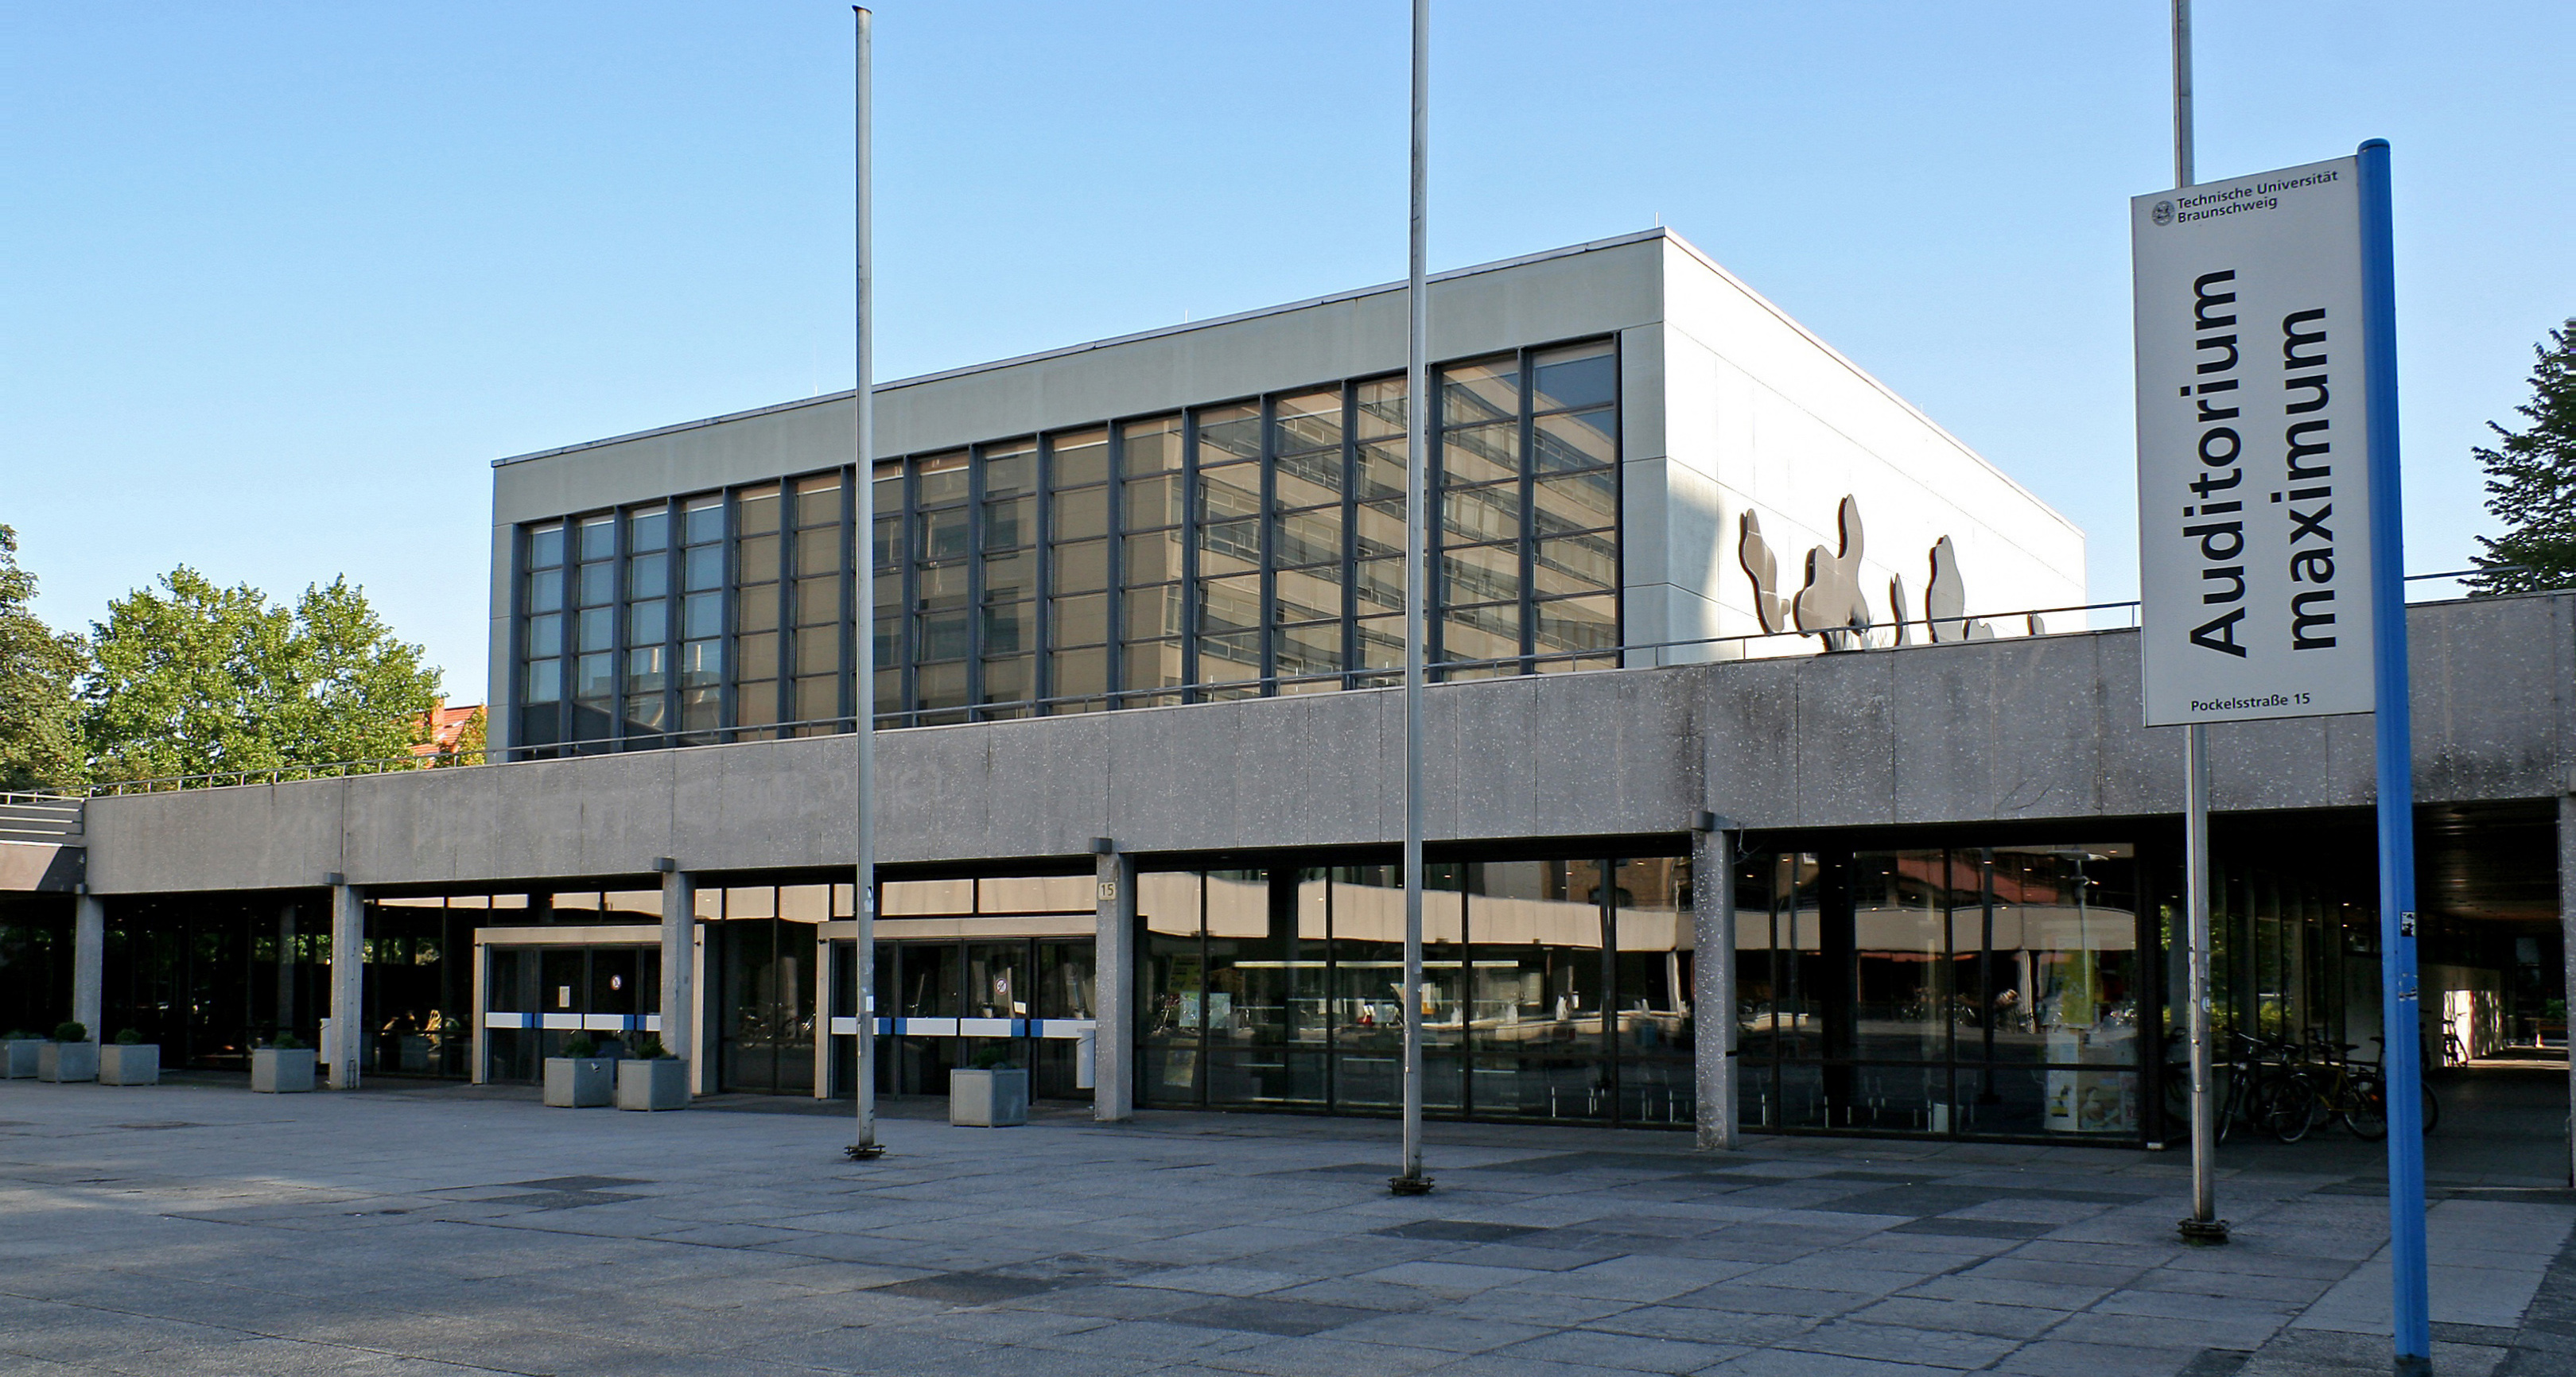
\includegraphics[width=\titlegraphicswidth]
    {titlepicture}}
\end{lstlisting}
\end{example}

Alternativ kann auch eine Höhenbeschränkung über die Längenangabe
\lstinline{\titlegraphicsheight} erfolgen. Dies ist besonders bei Grafiken
sinnvoll, deren Breite geringer als benötigt ist. Damit wird deren automatische
korrekte vertikale Skalierung sichergestellt.

\begin{example}
\begin{lstlisting}
\titlegraphic{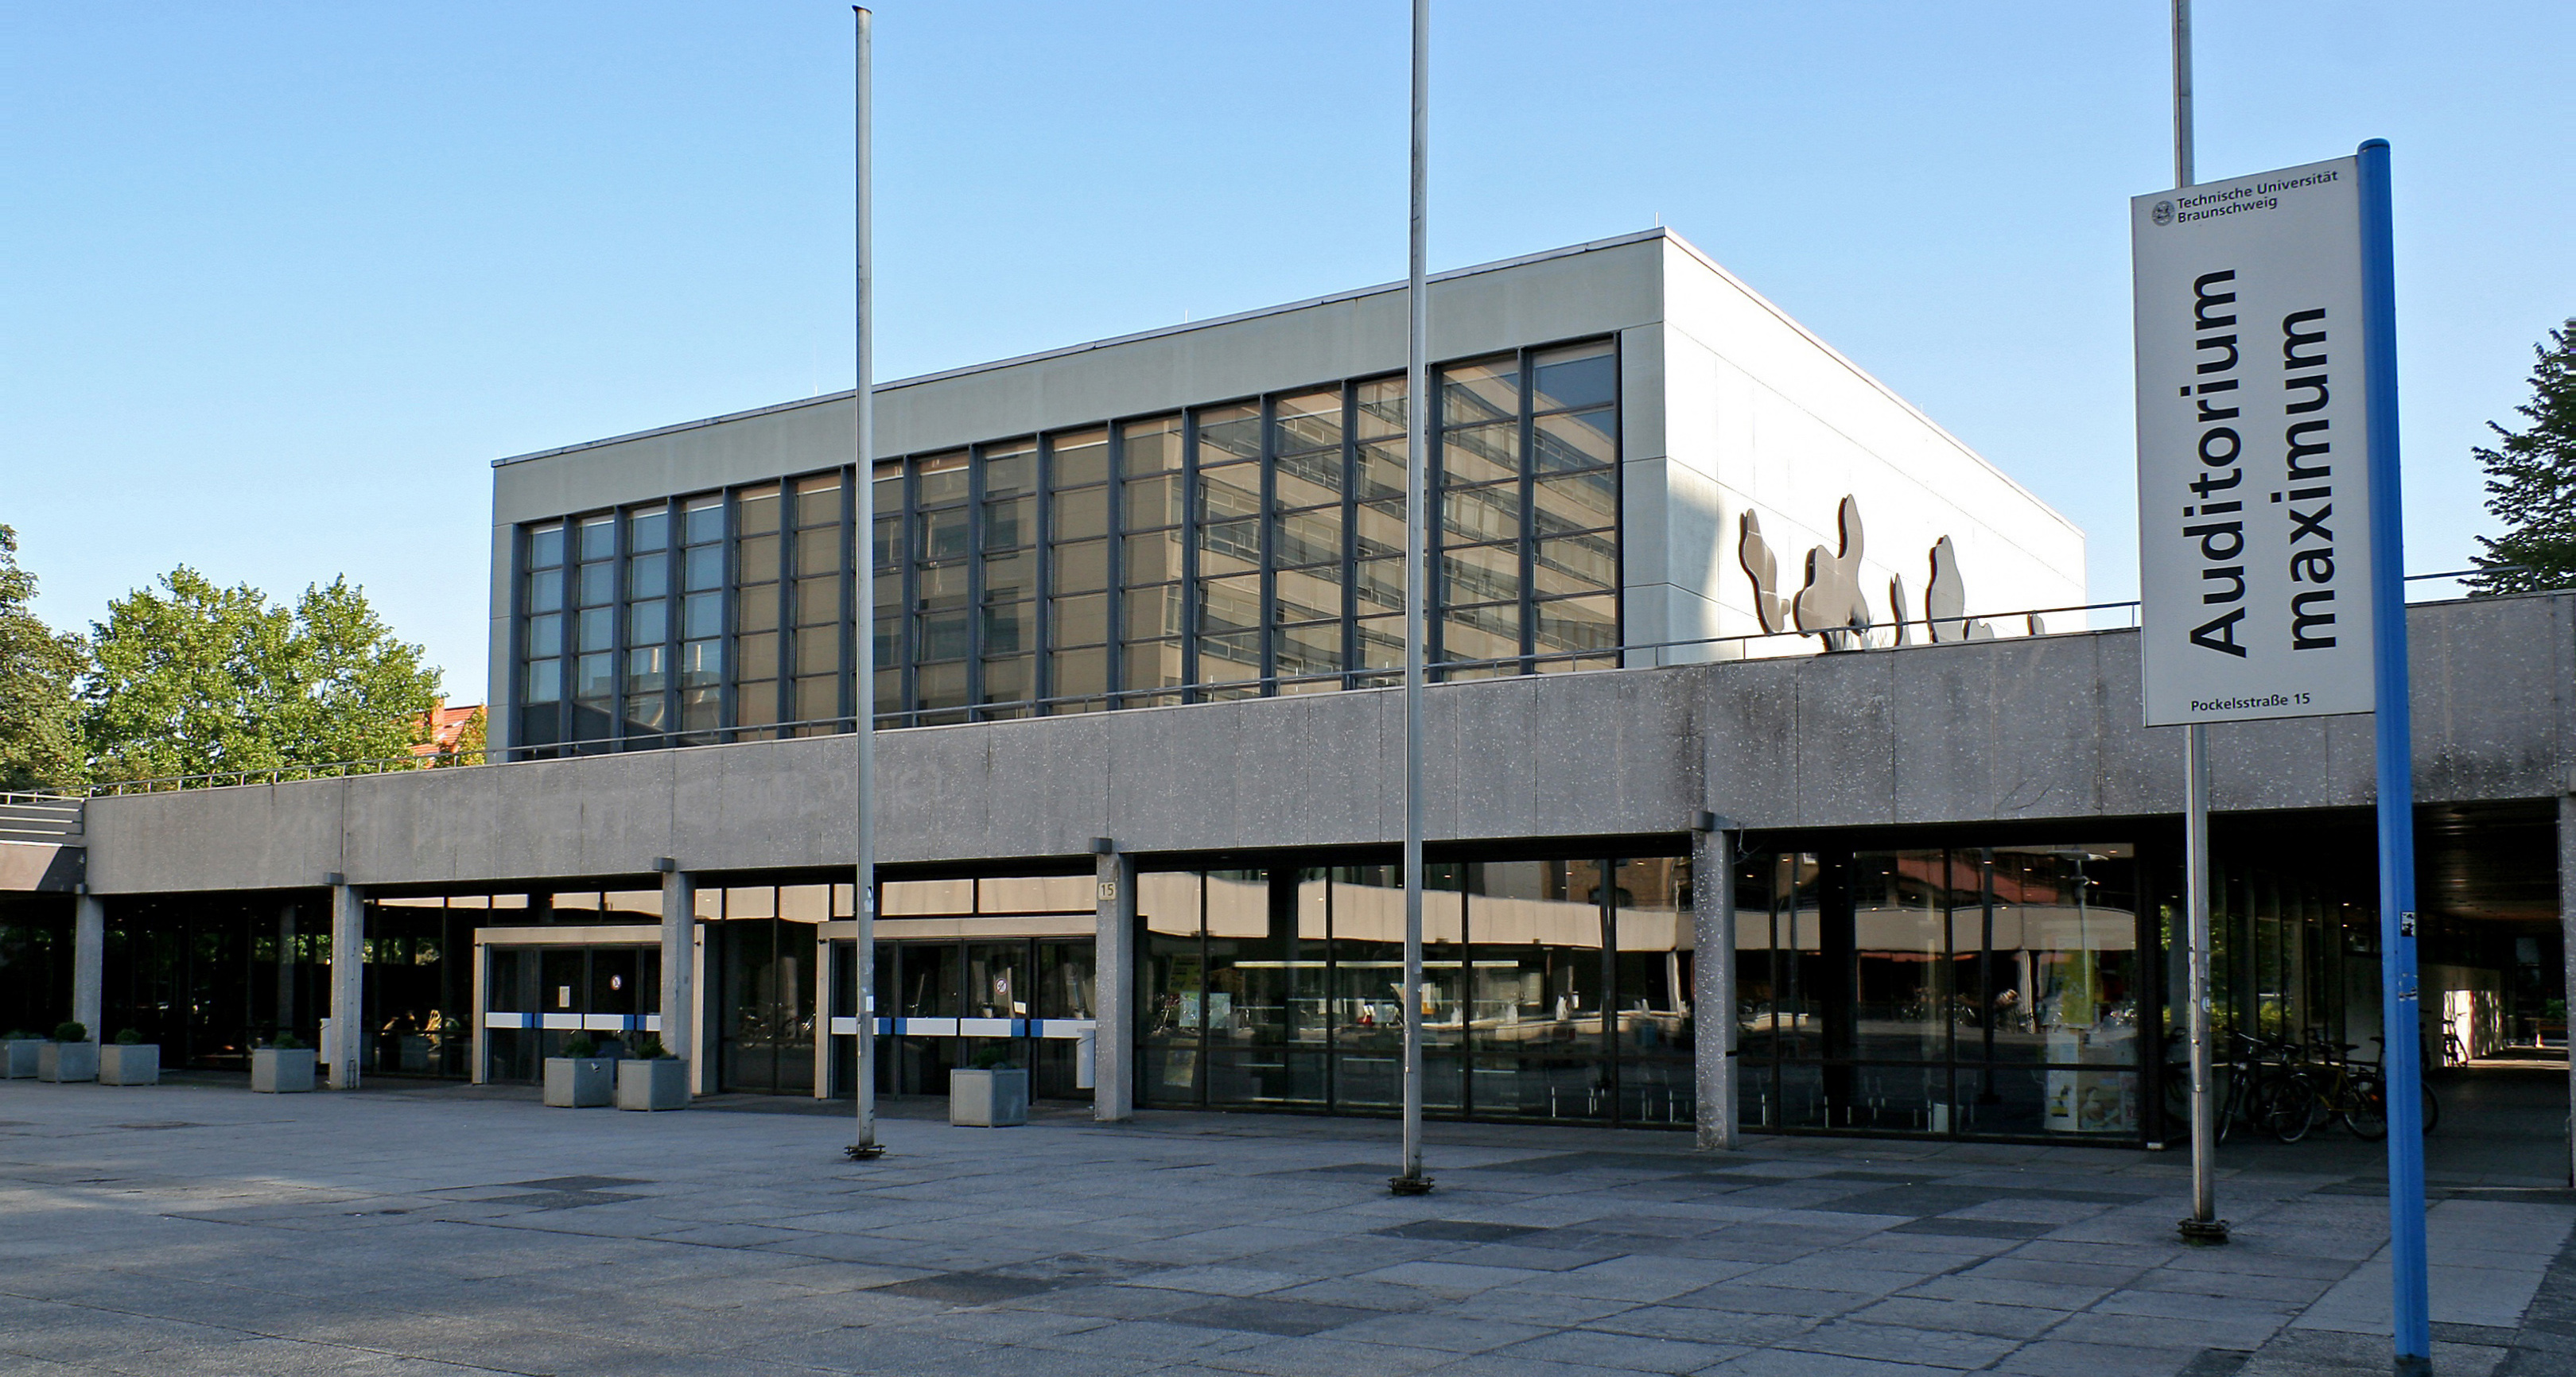
\includegraphics[height=\titlegraphicsheight]
    {titlepicture}}
\end{lstlisting}
\end{example}

\subsection{Logo}

Das mittels \lstinline{\logo} eingebundene Logo wird in der rechten oberen
Ecke des Absenderbereiches angezeigt und standardmäßig auch auf allen weiteren
Folien im Fußbereich, sofern nicht die Option \lstinline{nologoinfoot}
verwendet wird.

Die Verwendung von \lstinline{\logoheight} als Höhenbeschränkung für Grafiken
stellt deren automatische korrekte vertikale Skalierung sicher.
Das Seitenverhältnis der verwendeten Grafik-Datei ist dabei relativ
frei, sollte jedoch nach Möglichkeit und Gründen der Lesbarkeit breiter sein als
hoch.

\begin{example}
\begin{lstlisting}
\logo{
\includegraphics[height=\logoheight]{institut.jpg}}
\end{lstlisting}
\end{example}


\section{Inhaltsfolien}

Das Layout der Inhaltsfolien ist relativ schlicht und bietet viel Platz.
Die Überschrift ist im Kopfbereich grau hinterlegt und im Fußbereich der Folien
findet sich das TU-Logo, sowie eine rote Trennlinie.
Rechts unterhalb der Trennlinie wird, wenn definiert, das Logo angezeigt.
Ist dies nicht gewünscht, kann dies mit der Klassenoption
\lstinline{nologoinfoot} unterdrückt werden.

\begin{minipage}{0.5\textwidth}
\begin{verbatim}
\begin{frame}{Inhaltsseite}
  \begin{itemize}
    \item Hier steht der Inhalt
    \item Hier nicht
    \item Weitere Informationen
  \end{itemize}
\end{frame}
\end{verbatim}
\end{minipage}
\begin{minipage}{0.5\textwidth}
\fboxsep0mm
\fbox{\includegraphics[width=0.9\textwidth]{examples/inhaltsseite.pdf}}
\end{minipage}

\subsection{Hervorgehobene Folien}

Einzelne wichtige Folien können extra hervorgehoben werden. Diese werden mit
der Umgebung \lstinline{highlightframe} erzeugt. Dies hat einen breiteren und
rot hinterlegten Titelbereich zur Folge.

% \begin{example}
% \begin{lstlisting}
% \begin{highlightframe}{Wichtig}
% Diese Folie ist wichtig!
% \end{highlightframe}
% \end{lstlisting}
% \end{example}

\begin{minipage}{0.5\textwidth}
\begin{verbatim}
\begin{highlightframe}
  {Inhaltsseite -- Hervorgehoben}
  \begin{itemize}
    \item Hier steht der Inhalt
    \item Hier nicht
    \item Weitere Informationen
  \end{itemize}
\end{highlightframe}
\end{verbatim}
\end{minipage}
\begin{minipage}{0.5\textwidth}
\fboxsep0mm
\fbox{\includegraphics[width=0.9\textwidth]{%
  examples/inhaltsseite_hervorgehoben.pdf}}
\end{minipage}

\subsection{Fußzeile}

In der Fußzeile steht laut Vorgabe Datum und Seitenzahl.
Ist das einmal nicht gewollt, kann dies durch Angabe der Optionen
\lstinline{nopagenum} bzw. \lstinline{nodate} unterdrückt werden.

Autor und Titel kommen aus dem optionalen Argument von \lstinline{\author}
und \lstinline{\title}, sodass auch Kurztitel möglich sind.
Ändert man im Babel-Paket die Sprache, ändert sich auch automatisch
die Fußzeile (\textit{page} statt Seite, anderes Datumsformat).


\section{Skalierbarkeit}

Die beamer-Option \lstinline{aspectratio}, mit der die Präsentation auch auf
andere Seitenformate gebrachte werden kann, wird vom Layout generell
unterstützt, jedoch ist zu bedenken, dass dafür ein Titelbild in einem anderen
Seitenverhältnis benötigt wird, wenn es passend dargestellt werden soll
(siehe Tabelle \ref{tab:picratio}).


\chapter{Optionen und Befehle}

\section{Optionen}

Auflistung aller Theme-spezieller Optionen zur Übergabe and die
Dokumentenklasse.

\subsection{Kopf-/Fußbereich}

\begin{classoption}{nopagenum}
  Blendet die mitlaufende Seitenzählung im Fuß der Folie aus.
\end{classoption}

\begin{classoption}{nodate}
  Blendet das Datum im Fuß der Folie aus.
\end{classoption}

\begin{classoption}{tocinheader}
  Erzeugt ein mitlaufendes Inhaltsverzeichnis im Folienkopf,
  das auch zur Navigation im Dokument genutz werden kann
  (entsprechend der Standard-Beamer-Klassen).
  
  Angezeigt werden standardmäßig sections und subsections.
  Sollen nur sections angezeigt werden, bitte die Option
  \lstinline{nosubsectionsinheader} verwenden.
  
\end{classoption}

\begin{classoption}{tinytocinheader}
  Wie \lstinline{tocinheader}, jedoch mit kleinerer Schrift.

  Kann eingesetzt werden für den Fall, dass das mit \lstinline{tocinheader}
  erzeugte Inhaltsverzeichnis zu breit wirkt oder die Foliendimension
  überragt.
\end{classoption}

\begin{classoption}{widetoc}
  Horizontal gestreckte Version des mitlaufenden Inahltsverzeichnisses.
\end{classoption}

\begin{classoption}{narrowtoc}
  Horizontal gestauchte Version des mitlaufenden Inahltsverzeichnisses.
\end{classoption}

\begin{classoption}{nosubsectionsinheader}
  Deaktiviert die Anzeige von subsections im Header.
  
  Nur wirksam, wenn Option \lstinline{tocinheader} oder
  \lstinline{tinytocinheader} verwendet wird!
\end{classoption}

\begin{classoption}{nologoinfoot}
  Deaktiviert die Anzeige des Logos im Fußbereich.
\end{classoption}

\subsection{Farben}

\begin{classoption}{rgbprint}
  Ausgabe in RGB-Druckfraben
\end{classoption}

\begin{classoption}{cmyk}
  Ausgabe in CMYK-Farben.
\end{classoption}


% \begin{classoption}{mathserif}
%   Beschreibung
% \end{classoption}

% \begin{classoption}{fleqn}
%   Beschreibung
% \end{classoption}

% \begin{classoption}{minion}
%   Beschreibung
% \end{classoption}


\section{Befehle}

% \titlegraphicsheight
% \tuDefaultTitlegraphic

\subsection{Schriftgröße}

\begin{classoption}{9pt}
  Beschreibung
\end{classoption}

\begin{classoption}{10pt}
  Beschreibung
\end{classoption}

\begin{classoption}{11pt}
  Beschreibung
\end{classoption}

\begin{classoption}{12pt}
  Beschreibung
\end{classoption}

\begin{classoption}{14pt}
  Beschreibung
\end{classoption}


\chapter{Minimalbeispiel}

Im folgenden ist der Code eines Minimalbeispieles aufgeführt, zusammen mit den
daraus erzeugten Folien.

\begin{verbatim}
\documentclass{beamer}

\usetheme{TU-CD}
\usepackage[T1]{fontenc}
\usepackage[utf8x]{inputenc}

\title{Corporate Design}
\subtitle{Jetzt mit \LaTeX}
\author{Max Mustermann}
\titlegraphic{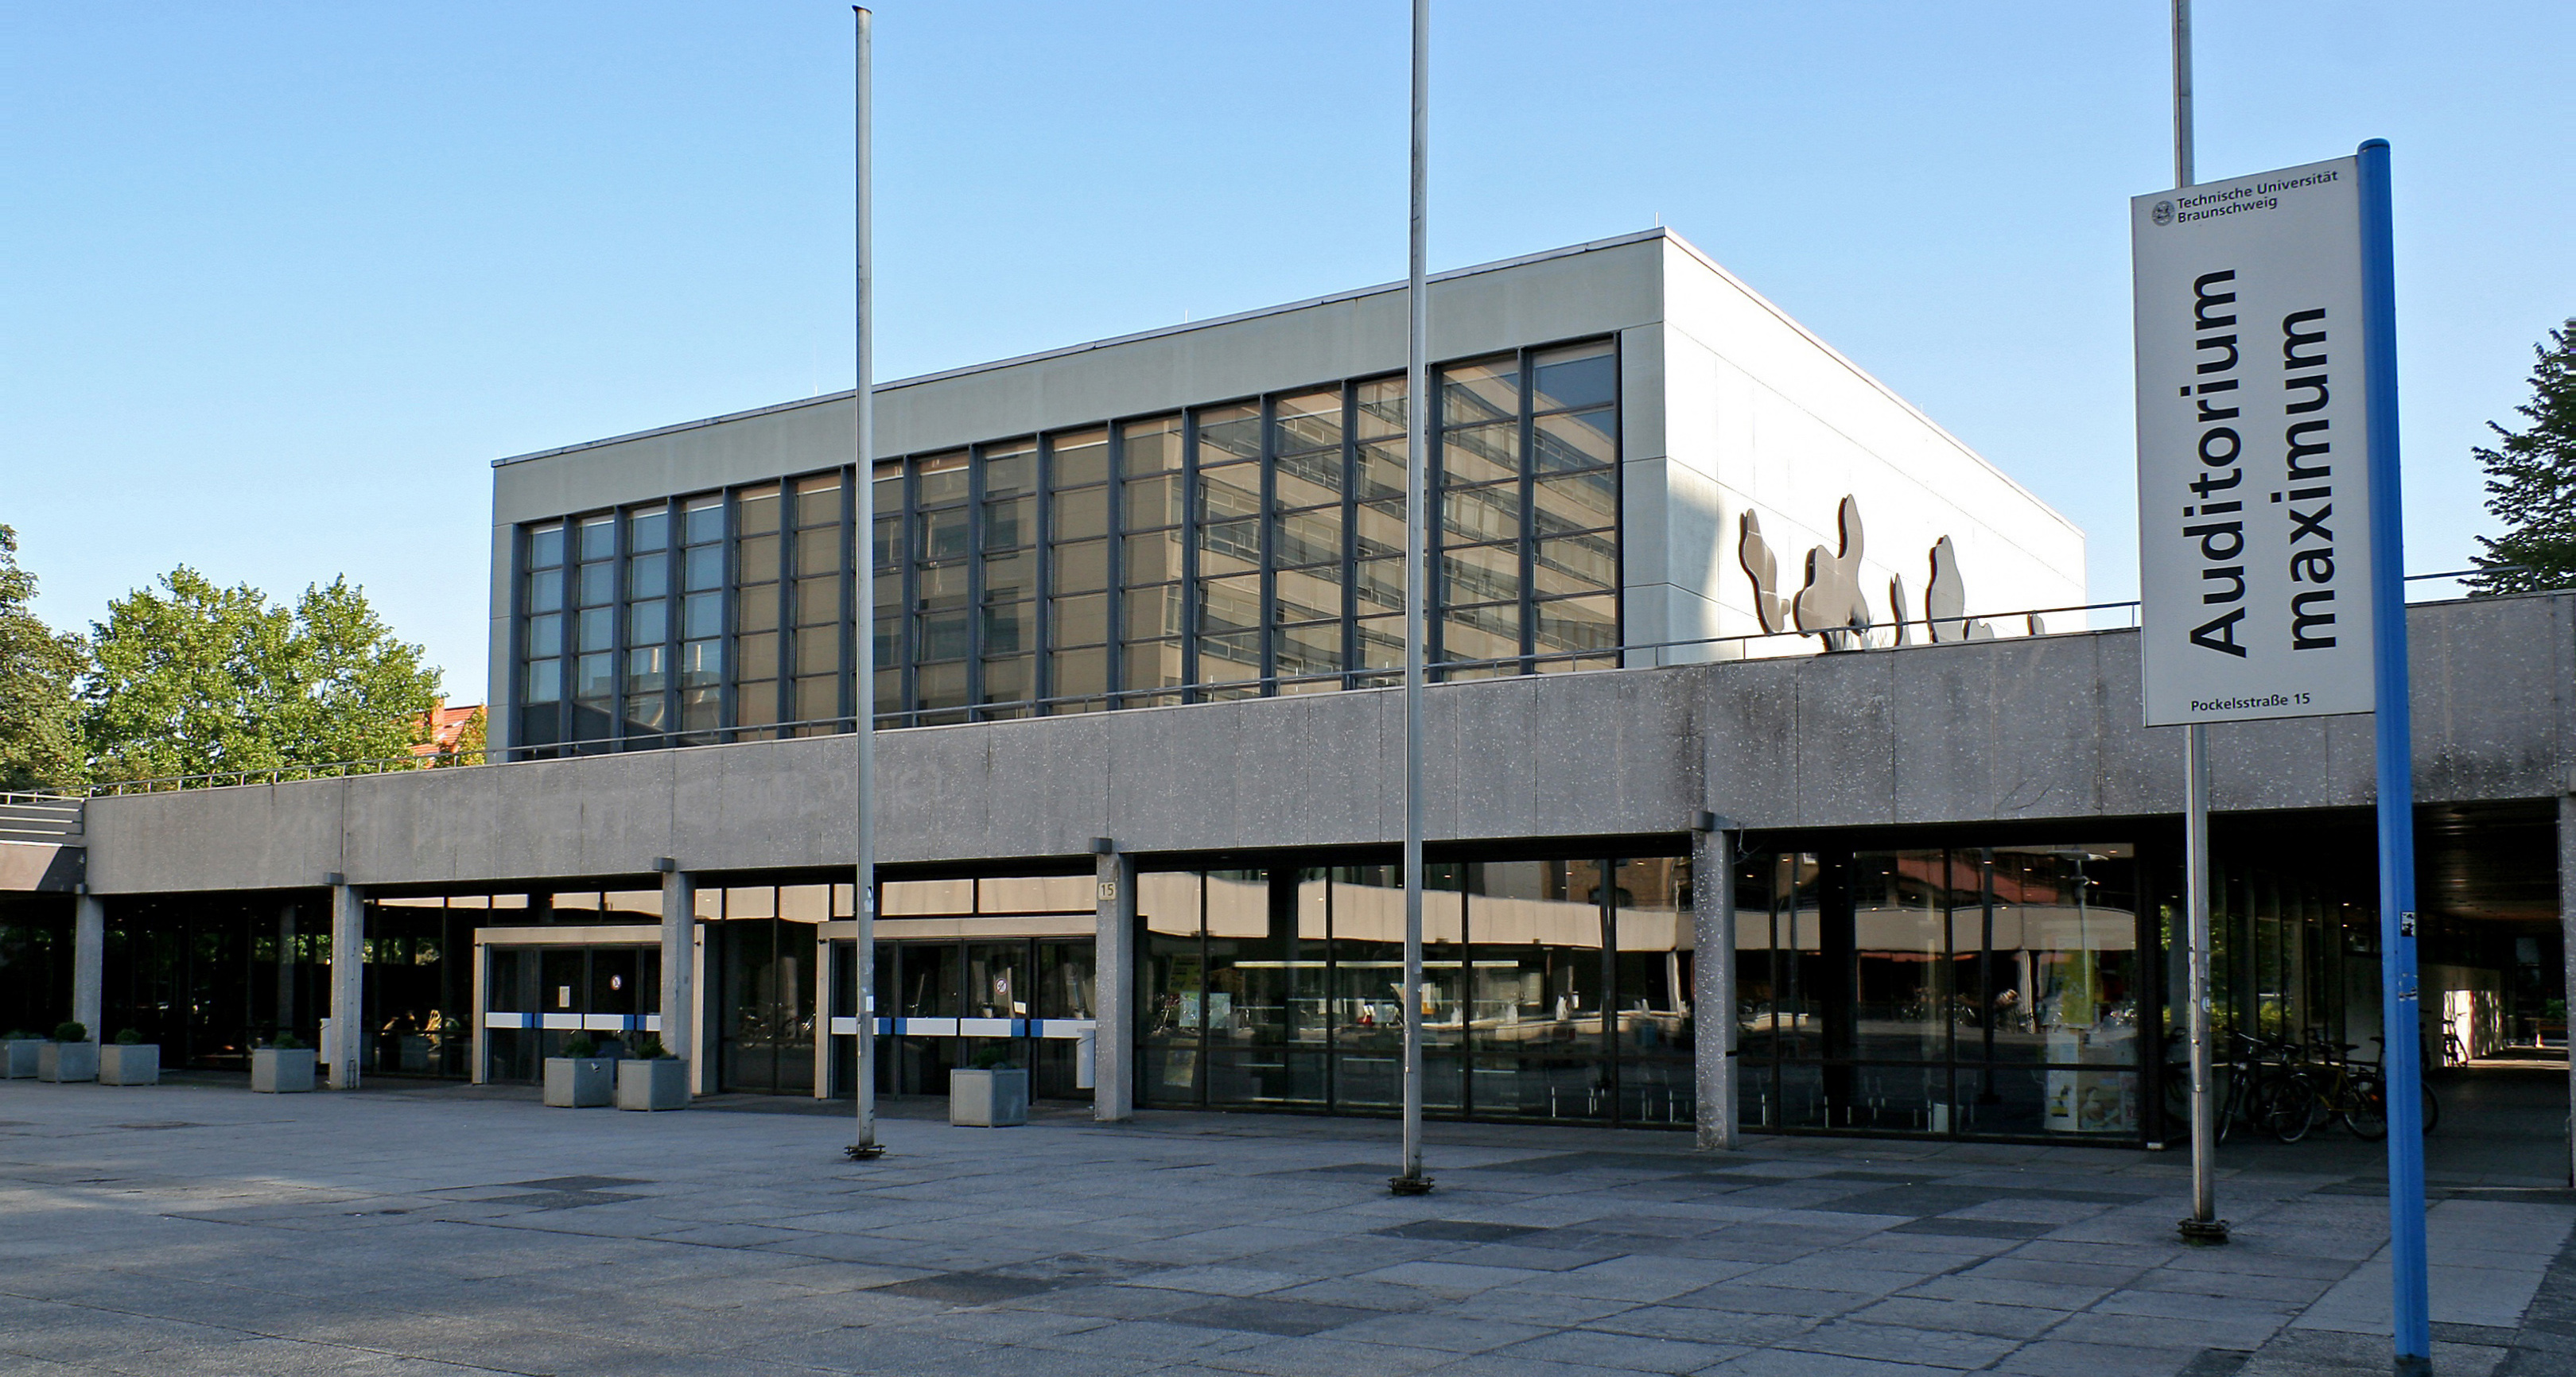
\includegraphics[width=\titlegraphicswidth]{titlepicture}}
\logo{
\includegraphics[height=\logoheight]{institut.jpg}}

\begin{document}

\begin{frame}[plain]
  \titlepage
\end{frame}

\begin{frame}{Inhaltsseite}
  \begin{itemize}
    \item Hier steht der Inhalt
    \item Hier nicht
    \item Weitere Informationen
  \end{itemize}
\end{frame}

\end{document}
\end{verbatim}

\begin{center}
  \fbox{\includegraphics[width=0.9\textwidth]{examples/titelseite.pdf}}

  \fbox{\includegraphics[width=0.9\textwidth]{examples/inhaltsseite.pdf}}
\end{center}
\end{document}